\section{Desenvolvimento da Estrutura Empresarial - Hyperion / MyMed}

\subsection*{Nome da Empresa e Aplicativo}
Empresa: Hyperion 
Aplicativo: MyMed

\subsection*{Missão}
Queremos oferecer uma solução tecnológica eficiente e humanizada para auxiliar cuidadores, asilos e casas de repouso na organização e administração dos cuidados com idosos, promovendo segurança, bem-estar e qualidade de vida aos pacientes.

\subsection*{Visão}
Desejamos ser referência nacional no desenvolvimento de tecnologias voltadas ao cuidado de idosos, contribuindo para uma sociedade mais atenta, organizada e respeitosa com a terceira idade.  

\subsection*{Valores}
Responsabilidade - garantir o funcionamento confiável da plataforma, priorizando a segurança nas rotinas de medicação e cuidados.  
Cuidado - fornecer meios e ferramentas para garantir a segurança e uma melhora no gerenciamento e cuidado da saúde de idosos. 

\subsection*{Descrição da Empresa}
Nosso principal objetivo é desenvolver uma plataforma de auxílio de gerenciamento de tratamentos de um usuário e/ou seus dependentes, alertando sobre estoque remanescente, consultas agendadas, registros de índice de pressão e/ou glicemia. com um desenvolvimento próximo ao usuário final, interface simples e soluções razoáveis em comparação com a concorrência. 

\section{Análise de Mercado}

\subsection*{Público-Alvo (persona)}
Cuidadores, geralmente cuidadores de pessoas da terceira idade, que passam seus dias de trabalho realizando tarefas exaustivas e que consomem grande parte do seu tempo.  O nome da nossa persona principal é Juliana. Juliana é uma cuidadora que trabalha em uma casa de repouso, onde ela tem cinco pacientes e está usando o MyMed para administrar o tratamento de seus pacientes, com enfoque em administrar as medicações e as consultas de cada paciente. 

\subsection*{Necessidades dos Usuários}
Uma melhor organização e gerenciamento dos tratamentos e medicações do paciente daquele cuidador, focando na centralização do monitoramento de recursos. Principalmente por conta de não existir programas de assistência aos cuidadores. 

Uma forma eficiente de guardar informações e emitir relatórios e acessar gráficos a partir de suas necessidades, como períodos, ocorrências e registros.

\subsection*{Concorrentes}
Medisafe:\\
 O que oferece de diferente: \\
- Gestão de medicamentos com lembretes e alertas. \\
- Compartilhamento básico de informações com familiares e cuidadores. /SNS24, Lively Mobile Plus/Lica, Hora do Lar/Américo Cuidador, Cuidar de Idosos/Mais Amor Cuidadores, Hugs Care e DoseApp.\\
 Diferencial da sua aplicação: 
-  Gráficos detalhados de adesão ao tratamento. \\
-  Análise de interações medicamentosas. \\
-  Recomendações personalizadas para o idoso e cuidador.\\

MyChart / SNS24:\\
 O que oferece de diferente: \\
- Agendamento e registro de consultas médicas.  \\
- Acesso a receitas e teleconsultas.\\
 Diferencial da sua aplicação: \\
-  Integração com sistemas locais de saúde.  \\
-  Análise preditiva de saúde.\\
-  Alertas personalizados para exames e consultas futuras. \\

Lively Mobile Plus / Lica:\\
 O que oferece de diferente:\\
-  Monitoramento de quedas e alertas emergenciais.\\
-  Monitoramento de sinais vitais em tempo real.\\
 Diferencial da sua aplicação:\\
-  Monitoramento contínuo com inteligência artificial para antecipar riscos.\\
-  Relatórios detalhados para familiares e cuidadores.\\

Hora do Lar / Américo Cuidador:\\
 O que oferece de diferente:\\
-  Gestão do cuidador profissional: contratação, controle de jornada e conformidade legal.\\
 Diferencial da sua aplicação:\\
-  Gestão integrada do idoso e do cuidador.\\
-  Dashboards multidimensionais que acompanham saúde, tarefas e bem-estar.\\

Cuidar de Idosos / Mais Amor Cuidadores:\\
 O que oferece de diferente:\\
-  Conteúdo educativo e dicas para cuidadores iniciantes.\\
 Diferencial da sua aplicação:\\
-  Conteúdo educativo integrado diretamente na plataforma.\\
-  Suporte em tempo real e canais de comunicação para dúvidas.\\

Apps de comunicação (ex: Hugs Care):\\
 O que oferece de diferente:\\
-  Troca de experiências entre cuidadores e familiares.\\
-  Comunicação simples e direta.\\
 Diferencial da sua aplicação:\\
-  Plataforma integrada para comunicação entre familiares, cuidadores e profissionais.\\
-  Histórico e notificações centralizadas para melhor acompanhamento.\\

DoseApp (código aberto):\\
 O que oferece de diferente:\\
-  Compartilhamento de informações sobre medicação e rotina.\\
-  Interface simples e acessível.\\
Diferencial da sua aplicação:\\
-  Interface intuitiva e multiplataforma (web e mobile).\\
-  Uso de inteligência artificial para personalização e automação de tarefas.\\
\subsection*{Diferenciais da Solução}
Temos como base do projeto o foco nos cuidadores, onde temos uma interface intuitiva, atraente e que centraliza as informações pertinentes aos pacientes, permitindo melhor compreensão do quadro do dependente, alertas e lembretes para melhor organização de tempo, relatórios personalizados sobre consultas e medicamentos, pesquisa de preços de medicamentos e desenvolvimento orientado à feedback do usuário. 

\section{Modelo de Negócio}
\begin{figure}[!htbp]
    \centering
    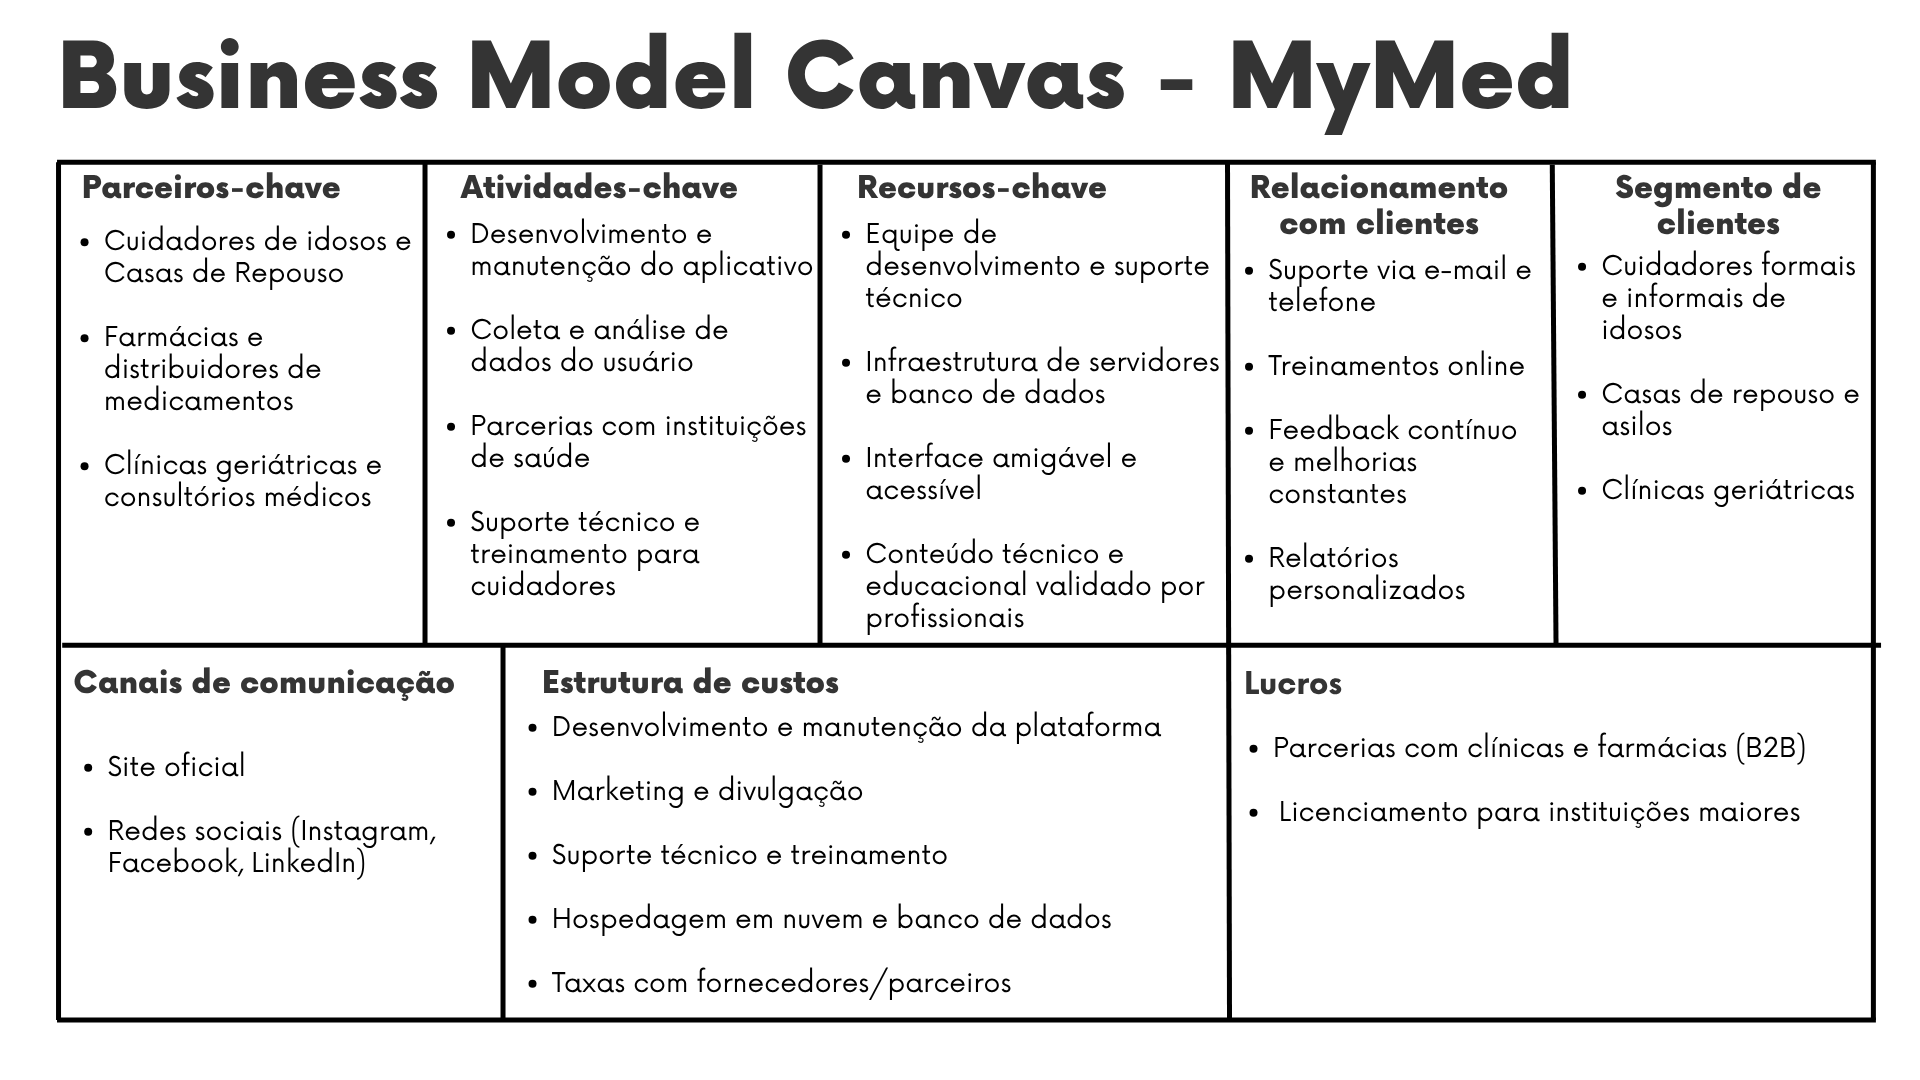
\includegraphics[width=0.75\linewidth]{Figuras/BMC.png}
    \caption{Business Model Canva - MyMed}
    \fonte{Autores.}
\end{figure}

\subsection*{Fonte de Receita}
Nosso sistema tem enfoque em ser acessível e oferece uma versão gratuita com anúncios, alcançando um público amplo. Para uma experiência aprimorada, a assinatura Premium remove anúncios e desbloqueia funcionalidades avançadas que exigem uma maior análise de dados ou poder de processamento. Este modelo de assinatura é importante para a sustentabilidade do projeto, permitindo investimento contínuo em pesquisa, desenvolvimento e infraestrutura, garantindo um serviço inovador e de alta qualidade.

\subsection*{Parcerias Principais e Recursos-chave}
Parcerias principais: Clínicas, farmácias, ONGs, planos de saúde, universidades; \\
Recursos-chave: Equipe de desenvolvedores, Experiência do usuário (UX) acessível, base de dados segura, notificações e suporte ao usuário contínuo; \\
Ativos estratégicos: Reputação, conteúdo educativo, comunidade ativa de cuidadores e divulgadores.\\


\section{Estratégia de Lançamento e Marketing}
No pré-lançamento, queremos disponibilizar uma versão beta do MyMed para familiarizar os usuários com a interface e estabelecer um canal contínuo de feedback para aprimoramento ao longo das próximas versões. A divulgação nesse período será realizada por meio de clínicas geriátricas, ONGs de saúde que trabalham com cuidadores e farmácias. A partir dos feedbacks, faremos uma análise se após aprimorar o projeto com as sugestões, podemos realizar o lançamento oficial, onde colocaremos o aplicativo nas lojas e disponibilizar o aplicativo para o público. Nosso foco no pós-lançamento é continuar investindo na pesquisa e desenvolvimento e aprimorar o aplicativo ao longo do tempo, com funcionalidades que mantenham o usuário engajado e fiéis ao nosso aplicativo. Nossas métricas de sucesso serão medidas através de número de downloads nas lojas de aplicativo, a retenção de usuários e o sucesso para realizar determinadas ações. \\\\
Como estratégia de aquisição de usuários, realizaremos o marketing de conteúdo através de redes sociais, campanhas pagas de baixo custo (Google Ads), permitir o uso do aplicativo de forma gratuita para casas de repouso, cuidadores ou farmácias locais, e App Store Optimization (Play Store, App Store). \\\\
Nossos canais de divulgação serão as clínicas geriátricas, ONGs de saúde, farmácias (com material impresso simples como flyers com QR code), casas de repouso, redes sociais (principalmente Instagram), Google Ads e Facebook Ads, e, caso possível, influenciadores digitais (preferencialmente cuidadores).\\\\

\section{Aspectos Técnicos e Operacionais}

\subsection*{Tecnologias Utilizadas}
Back-end: Java com SpringBoot, MySQL, hospedagem em Render e Google Cloud. \\
Front-end: Angular 19, PrimeNG, Auth0. \\
Versionamento: Git, GitHub, GitKraken. \\
Gestão: Jira e Google Drive.

\begin{figure}[h!]
    \centering
    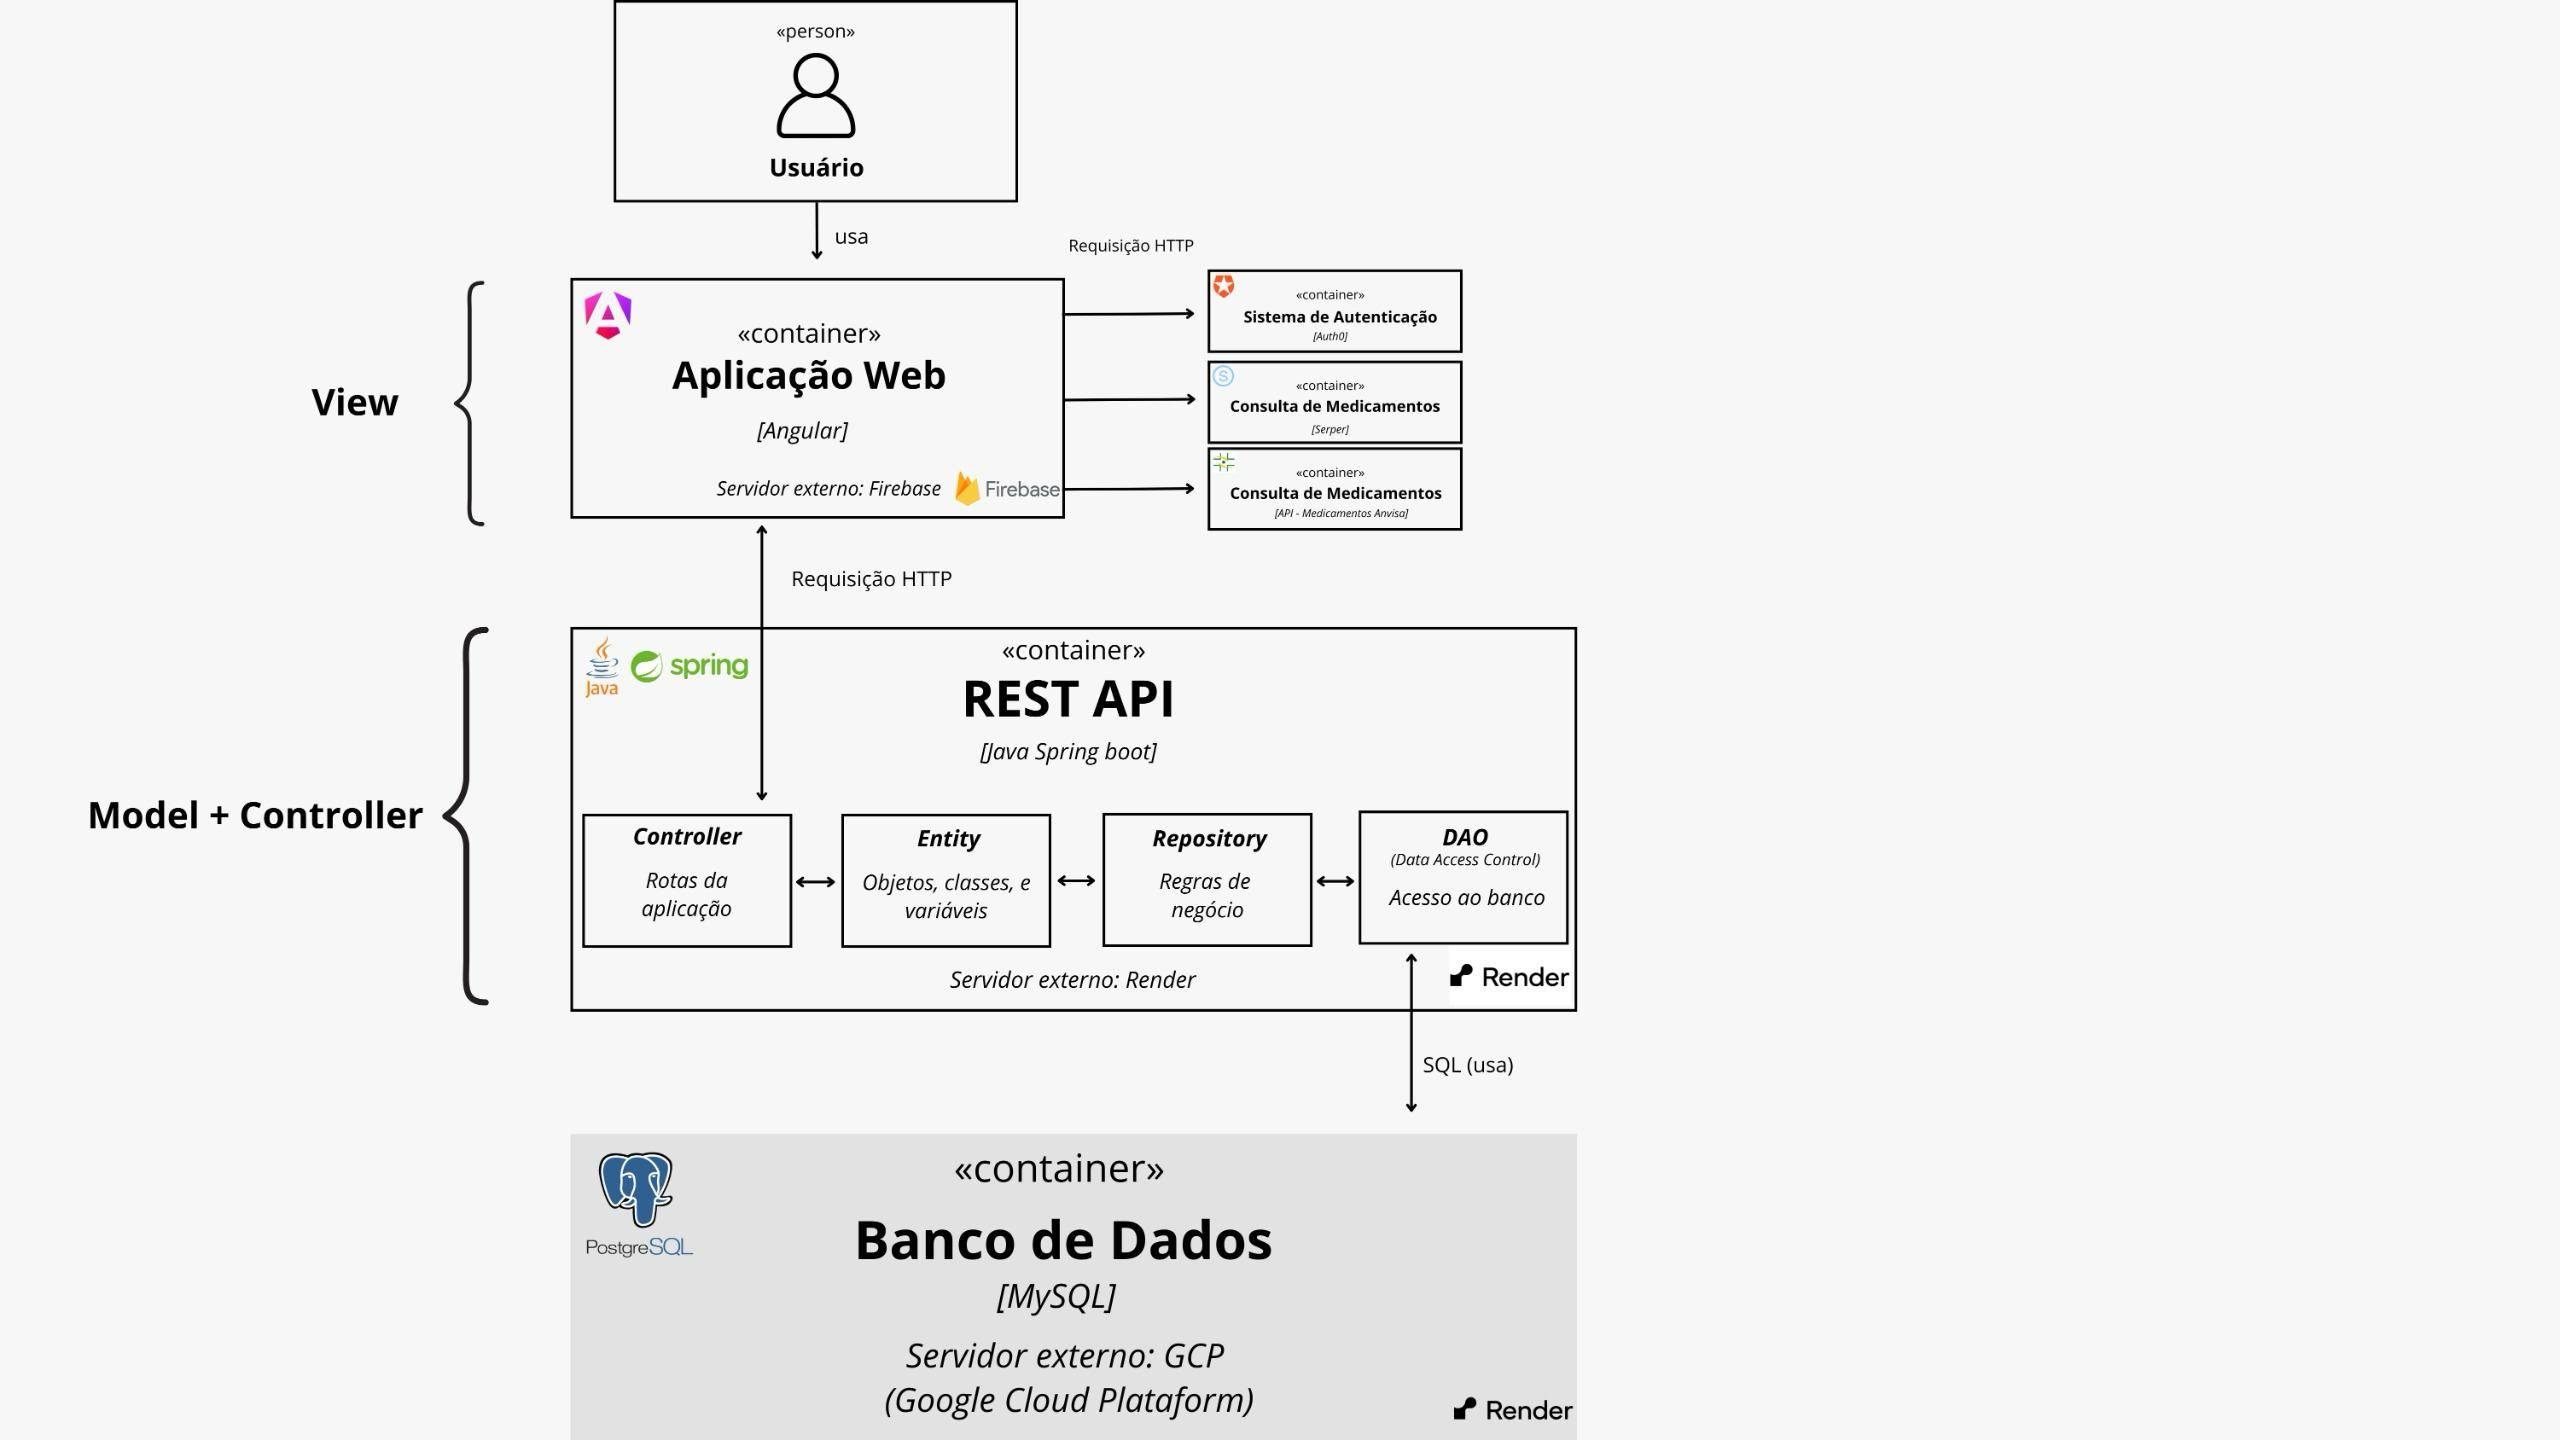
\includegraphics[width=1.5\textwidth]{Figuras/diagrama_de_software.jpeg}
    \caption{Diagrama de Arquitetura de Software}
    \label{fig:fluxo-comunicacao}
    \fonte{Autores.}
\end{figure}


\subsection*{Equipe e Funções}
A equipe e as funções de cada integrante são encontradas no \autoref{quadro_integrantes}.


\subsection*{Ferramentas de Desenvolvimento}
Editor: VSCode. \\
Versionamento: Git/GitHub. \\
Gestão: Jira. \\
Armazenamento: Google Drive.


\section{Viabilidade Econômica}

\subsection*{Custos Estimados}
Os custos estimados nos primeiros seis meses seriam de R\$50.000 a 60.000, considerando custos administrativos, marketing, servidores, design e desenvolvimento, mas se considerarmos que no início não teríamos um ‘salário’ dignamente posto, o custo cairia para R\$35.000 a 45.000. 